\section{E3NN}

\begin{frame}{E3NN: Density fitting}
  \begin{itemize}
    \item A consistent basis for all the charge density, not the case for DFT.
    \item {\color{red} \textbf{Density fitting}}: fit the density to a predefined basis set, def2-universal-JFIT\footnotemark.
  \end{itemize}
  \begin{equation*}
    \rho(\mathbf{r}) = \sum_b C_b \phi_b^{\text{basis}}(\mathbf{r}),
  \end{equation*}

  The objective function is to minimize:
    $\mathcal{L} = \frac{1}{N} \sum_i \left(C_b - \widehat{C_b}\right)^2$.
  \begin{itemize}
    \item 3 hidden layers.
    \item Input reps = 2x0e (2 channels l=0) with hydrogen ([1, 0])
    and oxygen ([0, 1]).
    \item Hidden reps = 125x0o + 125x0e + 40x1o + 40x1e + 25x2o + 25x2e + 15x3o + 15x3e.
    \item Output reps = 7x0e + 4x1e + 2x2e + 1x3e.
  \end{itemize}

  \footnotetext[6]{
    Rackers, Joshua A., et al. "Cracking the quantum scaling limit with machine
    learned electron densities." arXiv preprint arXiv:2201.03726 (2022).
  }
\end{frame}


\begin{frame}{The effect of cluster size on density prediction}
  This is one of the first lines of work:
  \begin{itemize}
    \item Does not train on large dataset for density prediction.
    \item Training on specific systems to push the frontier of quantum chemistry
    calculations.
  \end{itemize}
  The y-axis is the relative $L^1$-error.
  \begin{figure}
    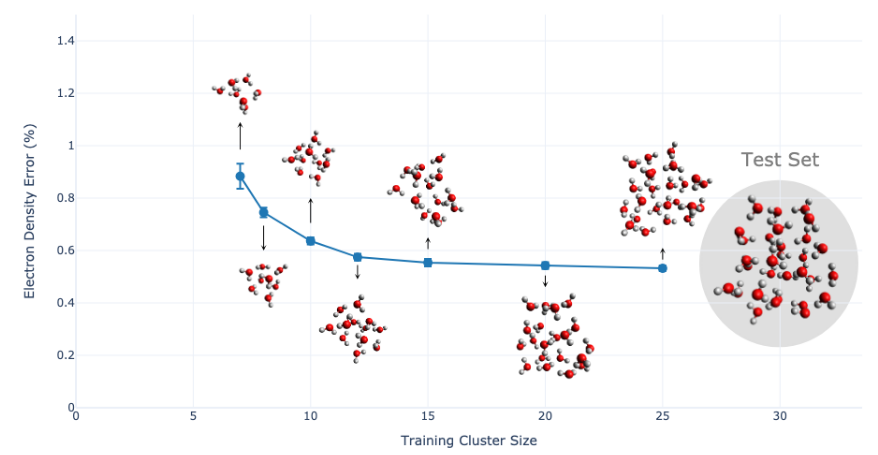
\includegraphics[width=0.6\textwidth]{figures/e3nn_2.jpg}
  \end{figure}
\end{frame}